\chapter{Introducción a los fundamentos de redes}
\subsubsection{Objetivos}
\begin{itemize}
    \item Conocer y comprender los principios básicos de las comunicaciones.
    \item Entender el diseño funiconal en capas de las redes y los conceptos y terminología fundamentales involucrados. 
    \item Comprender desde un punto de vista teórico-conceptual el modelo de referencia \acrshort{OSI} y su correspondencia con el modelo de capas usado en Internet.
\end{itemize}

\subsubsection{Introducción}
La arquitectura lógica de Internet está diseñada por capas. Veremos el modelo TCP/IP (aunque mencionaremos el modelo \acrshort{OSI}):
\begin{table}[h]
    \centering
    \begin{tabular}{|c|}
        \hline
        Aplicación que hace uso de la red\\ \hline
        Transporte \textbf{(TCP/UDP)} \\ \hline
        Red \textbf{(IP)} \\ \hline
        Enlace \\ \hline
        Física \\ \hline
    \end{tabular}
    \caption{Modelo de capas del protocolo TCP/IP.}
    \label{table:_tabla_de_capas}
\end{table}

Las dos últimas capas están implementadas en Hardware y las tres primeras en Software, también llamado \acrfull{NOS}. En la asignatura veremos las capas altas, las implementadas en software.

\section{Sistemas de comunicación y redes}

\begin{definicion}[Sistema de comunicación]
    Es una infraestructura (hw + sw) que permite el intercambio de información. Un sistema típico es el siguiente:
    \begin{itemize}
        \item Tenemos una fuente y un transmisor en un mismo equipo (que es el que va a mandar la información). La fuente genera la información y el transmisor adapta la información al medio.
        \item Después tenemos el canal de comunicación, el cual produce errores: ruidos, interferencias, diafonías (cuando hay muchos cables en paralelo juntos, puede suceder que la información de un cable se meta en otro)\ldots
        \item Al final tenemos un receptor y el destino (en un mismo equipo). El receptor adapta la información para el destino y éste espera los datos a recibir. 
    \end{itemize}
\end{definicion}


\subsection{Motivación para usar redes}
Para entender su uso hablaremos de la primera red de comunicaciones, que era una red de telefonía móvil. 
Cada usuario contaba con su línea de teléfono, que conectaba con una central de conmutación local, luego regional y luego nacional, la cual debía conectarse con la central local del destino. Se usaba conmutación de circuitos. 
\begin{itemize}
    \item Inicialmente se creaba un camino físico juntando cables, llamado circuito. 
    \item Era ineficiente porque no se está hablando todo el tiempo, y los tiempos de silencio el circuito se desaprovecha. 
    \item Era un problema de seguridad el mal funcionamiento de una central, pues dejaba a miles de teléfonos sin servicio. 
\end{itemize}

Si ahora pensamos en ordenadores (o equipos más generales, móviles, PCs, portátiles, móviles\ldots) en vez de móviles, y cambiamos las centrales de conmutación por routers, contamos con muchísimos caminos para conectar dos ordenadores, haciendo más segura la red.\\

En la actualidad ya no tenemos un camino físico, sino que son los routers quienes deciden por dónde enviar los paquetes y en qué momento. Estos tienen colas, lo que supone algo de retardo, pero tienen la ventaja de que se usa mucho mejor el canal y hay más seguridad, pues hay más de un camino.


\begin{definicion}[Red]
    Sistema de comunicación con sistemas finales o terminales autónomos (con capacidad para procesar información) que facilita el intercambio eficaz y transparente de información. Concretamente tenemos:
    \begin{itemize}
        \item\textbf{Hosts:} sistemas finales o terminales autónomos. Son los que transmiten y reciben datos. 
        \item\textbf{Subred:} infraestructura para el transporte de información, formada por líneas de transmisión y nodos o elementos de conmutación: routers y switches.   
    \end{itemize}
\end{definicion}

De una red esperamos:
\begin{itemize}
    \item Autonomía.
    \item Interconexión.
    \item Intercambio de información con eficacia y transparencia. 
\end{itemize}

En cuanto a medios de transmisión, originalmente se usaban cables de pares (pensados para transmitir $\unit[4]{kHz}$, la media de la voz humana), luego cables coaxiales, que mejoraron mucho; y fibra óptica que puede transmitir sin interferencias, por lo que es el mejor medio guiado existente. Los cables trenzados son para distancias más cortas, Ethernet por ejemplo. 

\subsection{Topologías de redes}

Dada una subred, su topología es el patrón de interconexión entre sus nodos. Las más relevantes las veremos a continuación.
\begin{description}
    \item[En bus:] Todos los nodos tienen acceso a un mismo medio, conocido como bus. Es la más sencilla, pero como el medio es común, todos intentan acceder y se producen colisiones. 
    \item[En anillo:] un círculo en el que tenemos los distintos nodos. Es similar al bus pues el medio es compartido. Una versión habitual es \textbf{token ring}, testigo de anillo, en el que se usa un testigo que se van pasando, de forma que así se evitan colisiones. 
    \item[En estrella:] todos están conectados a un centro principal, típicamente un switch. 

    A diferencia del bus, en este caso cada cable es independiente del resto. Si un PC pone algo en una toma el resto no lo escuchan. Cada línea tienen una cola para guardar a dónde enviar los paquetes y el switch tiene un procesador que coge los paquetes de dichas colas y los envían a las salidas. Es una topología mucho más segura por el hecho de no compartir el medio. 

    \item[En árbol:] típica en redes empresariales. Se suele estructurar en tres niveles:
    \begin{itemize}
        \item Primer nivel: red troncal.
        \item Segundo nivel: red de división.
        \item Tercer nivel: red de acceso. 
    \end{itemize}
    Los equipos de primer y segundo nivel suelen ser switches.
    
    Como potencial riesgo, pueden aparecer ciclos en el árbol. Ethernet no tiene ningún mecanismo para evitar que un paquete se mueva en círculo, lo que echaría la red abajo. El protocolo \acrfull{STP} elimina en cualquier topología los enlaces redundantes que formen bucles.

    \item[Mallada:] todos los nodos están conectados entre sí por medios independientes.
    
    Es muy fiable, ya que si se cae un enlace tienes más caminos para llegar a tu destino. No obstante, no es escalable, ya que si metemos un $n-$ésimo nodo hay que meter $n-1$ enlaces. Para redes pequeñas es de gran utilidad.

    Dentro de una empresa, la red troncal puede seguir esta topología para evitar caídas importantes. 

    \item[Híbrida:] se usa una mezcla de todas. Es la más utilizada.   
\end{description}

En cuanto a las topologías que comparten el medio, para evitar el ya mencionado problema de las colisiones, se usan los dos protocolos que veremos a continuación.
\begin{definicion}[CSMA/CD]
    El protocolo \acrfull{CSMA/CD} se encarga de detectar colisiones en topologías que comparten el medio, y dar error en caso de que se produzcan. Estas se detectan comprobando si lo que hay en el bus es lo que se acaba de poner.

    Es el protocolo que usa Ethernet.
\end{definicion}

\begin{definicion}[CSMA/CA]
    El protocolo \acrfull{CSMA/CA} se encarga de evitar colisiones en topologías que comparten el medio. Para ello, primero escucha el medio y, si no hay ningún mensaje, envía el mensaje. Si no recibe confirmación, hay colisión.

    Es el protocolo que usa Wi-Fi.
\end{definicion}


\subsection{Clasificación de redes}
\begin{description}
    \item[Según tamaño y extensión:] \
    \begin{itemize}
        \item \acrfull{PAN}: Red de área personal. Incluye todo lo que puede tener una persona: relojes, portátiles, cascos\ldots
        \item \acrfull{LAN}: Red de área local. Abarca unas decenas de metros,suele ser un mismo edificio. 
        \item \acrfull{MAN}: Red de área metropolitana. Se usa para conectar un campus o una ciudad. 
        \item \acrfull{WAN}.: Red de área extensa. Son redes desponibles en todo el país, como las redes telefónicas.
    \end{itemize}
    \item[Según tecnología de transmisión:]\
    \begin{itemize}
        \item Difusión: lo que pone un nodo en el medio le llega a todos. Ejemplo de esto es un HUB\@.
        \item Punto a punto: Cada nodo solo está unido a otro. Ejemplo de esto es un switch.
    \end{itemize}
    \item[Según el tipo de tranferencia de datos:] \
    \begin{itemize}
        \item Simple: solo transmite o recibe. Por ejemplo los TDT (para que una televisión analógica reciba señal digital).
        \item Half-duplex: transmite y recibe, pero no simultáneamente. Por ejemplo el Wi-Fi, aunque como cambia muy rápido  no nos damos cuenta.
        \item Full-duplex: transmite y recibe simultáneamente. Por ejemplo, Ethernet. 
    \end{itemize}
\end{description}

\subsection{Nomenclatura típica en figuras (Iconos)}
\begin{description}
    \item[HUB:] es un concentrador: permite centralizar los nodos de una red de computadoras. Se implementa mediante un bus.
    \item[Switch:] tiene muchas bocas y conecta dispositivos dentro de la misma red \acrshort{LAN}. Funciona en el nivel de enlace (nivel 2).
    \item[Bridge:] funciona como un switch, pero uniendo tecnologías distintas. También funciona en el nivel de enlace.
    \item[Router:] tiene pocas bocas, y se usa para conectar distintas redes. 
    \item[Cortafuegos:] bloquea el acceso no autorizado a una red, permitiendo tan solo el autorizado. 
    \item[NAT:] dispotivo en el que se ejecuta el protocolo \acrfull{NAT}, que permite que una red privada pueda acceder a Internet. Se explicará más adelante.
    \item[Switch multicapa\footnote{No se verá en la asignatura.}:] todas las bocas de un switch pertenecen a la misma \acrshort{LAN}, pero esto a veces no nos interesa. Podemos hacer distintas redes virtuales (\acrshort{VLAN}) dividiendo un mismo switch en varias redes, permitiéndonos esto conectar dos switches distintos dentro de la misma \acrshort{VLAN}. Esto no nos permite movernos por distintas redes en el mismo switch, ya habría que pasar por un router al necesitar movernos a nivel de red para cambiar de red.
    
    Esta es la funcionalidad que sí se puede hacer con un switch multicapa, no necesitar pasar por un router para cambiar de red.
\end{description}
% // TODO: Arturo. Añadir iconos?

\section{Diseño y estandarización de redes}

La idea principal que se sigue al diseñar redes es solucionar los problemas en capas. Se estandarizan Modelos de Referencia (no son implementaciones, solo una referencia), en los que se definen las distintas capas y las funcionalidades de cada una. Los principios que se siguen son que las funcionalidades distintas tienen que estar en distintas capas y minimizar el flujo de información entre las capas.\\

A continuación detallamos las capas de los modelos de referencia más importantes, junto a las funcionalidades de cada una y los problemas que han de solventar.
\begin{description}
    \item [Capa física:] se encarga de transmitir los datos. Hay distintos tipos de codificaciones para enviar bits de información.
    \item [Capa de enlace:] se encarga de los mecanismos de acceso al medio. Si hay un medio común, antes de transmitir datos tiene que asegurarse de que ningún equipo está transmitiendo. Suele seguir dos protocolos: 
        \begin{itemize}
            \item \acrfull{MAC}, control de acceso al medio.
            \item \acrfull{LLC}, control de acceso lógico para las primeras retransmisiones. Si algún paquete llega mal, retransmite varias veces. 
        \end{itemize}
    
    \item [Capa de red:] una vez llegado a este punto, se asume que no han habido colisiones en la comunicación. Esta capa se encarga principalmente de: 
        \begin{itemize}
            \item El direccionamiento: saber dar una dirección y tener un identificador dentro de la red. 
            \item El encaminamiento: saber cómo llegar al destino. 
        \end{itemize}

    \item [Capa de transporte:] se encarga de recuperar los paquetes que en la capa de enlace no se ha podido. Es la capa encargada de la fiabilidad. 
        \begin{itemize}
            \item Corrige errores.
            \item Gestiona la congestión de la red.
            \item Control de flujos: si hay un receptor más lento que el emisor, debe decirle al emisor que disminuya la velocidad de emisión, para adecuarse a la del receptor. 
        \end{itemize}
    Además se encarga de la multiplexación de datos: mediante puertos (los veremos más adelante) le indica al SO a qué aplicación corresponde cada paquete. 
    \item [Capa de aplicación:] los clientes y los servidores deben buscar alguna forma de comunicarse. 
\end{description}

Los dos modelos de referencia más importantes son el \acrshort{OSI} y el TCP/IP, que describiremos a continuación.
\subsection{Modelo OSI vs TCP/IP}
\begin{table}[H]
\centering
\begin{tabular}{|c|}
    \hline
    Aplicación \\\hline
    Presentación \\\hline
    Sesión \\ \hline
    Transporte \\ \hline
    Red \\\hline
    Enlace \\\hline
    Física \\\hline
\end{tabular}
\caption{Modelo OSI.}
\label{tab:mod_osi}
\end{table}

\begin{table}[H]
\centering
\begin{tabular}{|c|}
    \hline
    Aplicación \\\hline
    Transporte \\ \hline
    Red \\\hline
    Red subyacente \\\hline
\end{tabular}
\caption{Modelo TCP/IP.}
\label{tab:mod_tcp}
\end{table}

El modelo \acrfull{OSI} fue propuesto por la \acrshort{ISO} y el TCP/IP por el \acrshort{IETF}. Las tres primeras capas del modelo \acrshort{OSI} se corresponden con la capa de aplicación, y las dos última con la red subyacente, que es la parte física. Esta última en el modelo TCP/IP depende un poco de la tecnología está implementada de una forma u otra, pero la comunicación con la capa de red no puede variar, pues la capa de red si está estandarizada. 

\begin{itemize}
    \item Las capas físicas solo se encargan de hacer la primera conexión.
    \item La capa de red, salto a salto se encarga de llegar al destino, usando routers y sus tablas de encaminamiento. 
    \item Una vez hecho el encaminamiento, las capas superiores son solo de los extremos, son los computadores de los extremos los que se comunican. 
    \item Por tanto, los computadores tienen las 5 capas (en el caso de TCP/IP) y los routers solo las 3 más bajas. 
\end{itemize}


\section{Terminología, conceptos y servicios} \label{sec:terminologia}

\begin{figure}
    \centering
    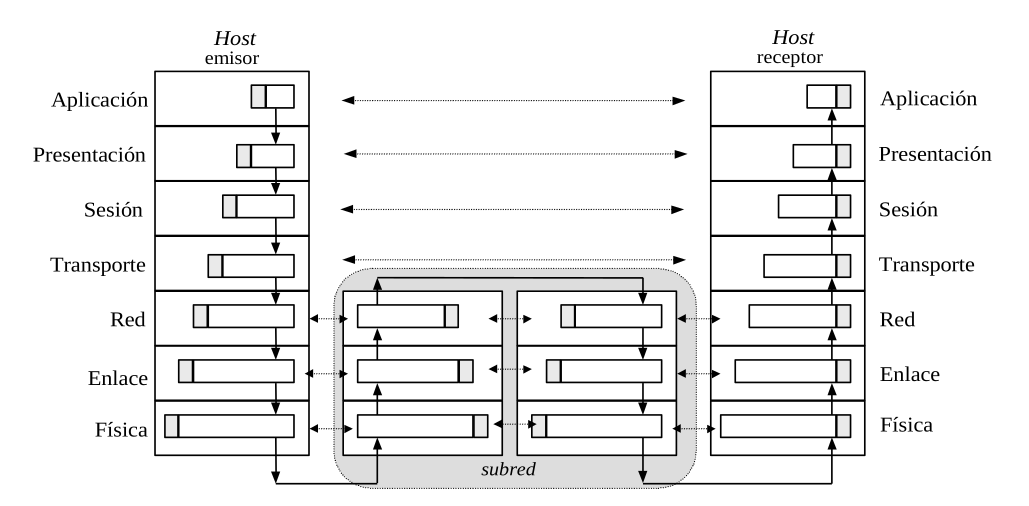
\includegraphics[width=0.8\linewidth]{./images/comunicacionHosts.png}
    \caption{Comunicación real frente a comunicación virtual.}
    \label{fig:comHosts}
\end{figure}

En la Figura~\ref{fig:comHosts} vemos el camino que siguen los datos que le manda un emisor a un receptor. A la hora de emitir, cada capa recibe los datos de la capa superior, conocidos como Unidad de Datos de Servicio (\acrfull{SDU}), y le añade una cabecera, formando la Unidad de Datos de Paquete (\acrfull{PDU}). Decimos que los datos de la capa superior se han \emph{encapsulado} en la capa inferior. Por tanto, cada capa envía el \acrshort{PDU} a la capa inferior convirtiéndose en el \acrshort{SDU} de la capa inferior. La capa física, al no tener capa inferior, manda señales eléctricas en vez de bits. \\

Por otra parte, en la recepción, cada capa recibe de la inferior el \acrshort{PDU}, al cual le quita la cabecera quedándose con el \acrshort{SDU}. En función de la cabecera, se estudia qué ha de acerse en cada capa y, posteriormente, se envía a la capa superior.\\

La información que se envía desde un host a otro ha de pasar por todas las capas para llegar al destino, lo que se conoce como \emph{comunicación real} o vertical, y viene representada en la Figura~\ref{fig:comHosts} por las flechas continuas. No obstante, y tan solo en sentido abstracto, decimos que nos capas del mismo tipo en distintos equipos hablan entre sí, lo que se conoce como \emph{comunicación virtual} u horizontal, y viene representada en la Figura~\ref{fig:comHosts} por las flechas discontinuas. Esta comunicación virtual, como ya hemos mencionado, no es directa, sino que se realiza a través de recursos que nos proporcionan otras capas adyacentes.\\

Además de las definiciones que acabamos de dar, otros términos relevantes son los siguientes:
\begin{description}
    \item [Entidad de nivel $n$:] entidad que se encuentra en la capa $n-$ésima.
    \item [Entidades pares:] entidades de la misma capa, que se comunican horizontalmente entre sí.
    \item [Protocolo:] reglas que describen cómo han de comunicarse las entidades pares. En ellos, se especifican los paquetes que se mandan, etc.
    \item [Interfaz:] a diferencia del protocolo, que se refiere a cómo se comunican las entidades pares, la interfaz se refiere a cómo se comunican las entidades de capas adyacentes.
    \item [\acrfull{SAP}:] punto de acceso al servicio. Es un punto específico en la interfaz entre dos capas donde se proporciona un servicio.
    \item [Servicio:] conjunto de funciones que una capa proporciona a la capa superior.
    \item [Capa proveedora/usuaria del servicio:] en la comunicación vertical, la capa que proporciona el servicio es la proveedora, y la que lo usa es la usuaria.
    \item [Pila de protocolos:] conjunto de protocolos que se usan en cada capa.
    \item [Arquitectura de red:] modelo de referencia, junto a la pila de protocolos.
\end{description}





Otro concepto importante es el de \emph{retardo}, que describireos a continuación.
\subsection{Retardos en la comunicación}
Supongamos que queremos transmitir un paquete entre dos equipos (terminales), por medio de otro, un router. Veamos los retardos que tenemos en la comunicación. 
\begin{enumerate}
    \item En primer lugar, hemos de considerar el \textbf{tiempo de transmisión}, que es el tiempo que se tarda en poner el paquete en el medio.
    
    Si el tamaño del paquete es de $\unit[L]{Bytes}$ y la velocidad de transmisión es de $\unit[v_t]{bps}$, el tiempo de transmisión $t_t$ es de:
    \begin{equation*}
        t_t = \unit[\frac{L\cdot 8}{v_t}]{s}
    \end{equation*}

    La velocidad de transmisión depende exclusivamente de la tarjeta de red.

    \item En segundo lugar, tenemos el \textbf{tiempo de propagación}, que es el tiempo desde que se escribe el primer bit en el medio hasta que llega este primer bit al siguiente equipo.
    
    Este tiempo depende de la distancia entre los equipos y de la velocidad de transmisión, que depende del medio. En el caso de una transmisión inalámbrica, la velocidad de transmisión es la velocidad de la luz, mientras que en una transmisión por cable suele ser de $\nicefrac{2}{3}$ de la velocidad de la luz.

    Si la distancia entre los equipos es de $\unit[d]{m}$ y la velocidad de transmisión es de $\unitfrac[v_p]{m}{s}$, el tiempo de propagación $t_p$ es de:
    \begin{equation*}
        t_p = \unit[\frac{d}{v_p}]{s}
    \end{equation*}

    \item En tercer lugar, tenemos el tiempo que se encuentra en el equipo intermedio, en nuestro caso el router. Cuando el paquete llega al equipo intermedio, éste lo mete en una cola hasta que pueda procesarlo. El tiempo que el paquete está en la cola depende se conoce como \textbf{tiempo de cola}, y depende de la situación del equipo. Además, el equipo ha de procesar el paquete, lo que le lleva un tiempo conocido como \textbf{tiempo de procesamiento}, que suele ser del orden de milisegundos. Por último, y para poder continuar con la comunicación, el equipo ha de obtener acceso al medio, lo que le lleva un tiempo conocido como \textbf{tiempo de acceso al medio}.
    
    Por tanto, el tiempo que el paquete está en el equipo intermedio es la suma de estos tres tiempos.

    \item Por último, la comunicación deberá continuar, por lo que se obtienen nuevos retardos de transmisión, propagación, etc. No obstante, en estos casos, estos no serán los mismos, pues la distancia entre equipos, tarjetas de red, etc., serán distintos.
\end{enumerate}

% // TODO: Arturo. Gráfica de los tiempos

\subsection{Tipos de servicios}
Relacionado con el nivel de transporte, hay dos clasificaciones importantes:
\begin{description}
    \item[Según la conexión:] En función de si, antes de enviar un paquete, se comprueba que el otro equipo esté encendido o no, tenemos dos tipos de servicios:
    \begin{itemize}
        \item \acrfull{SOC}: sí se comprueba.
        \item \acrfull{SNOC}: no se comprueba.
    \end{itemize}

    \item[Según la fiabilidad:] En función de si se asegura que todo funcione bien o no, (por ejemplo, que todos los bits de un archivo estén bien), tenemos dos tipos de servicios:
    \begin{itemize}
        \item Fiable: se asegura de que todo funcione bien. Si algo falla, la conexión se termina.
        \item No fiable: no comprueba que todo funcione bien. La finalidad de estos protocolos es ser rápidos.
    \end{itemize}

    Para tener un protocolo fiable, contamos con los siguientes mecanismos:
    \begin{itemize}
        \item Control de conexión. Ser fiable implica ser orientado a conexión.
        \item Control de errores.
        \item Control de congestión. Hablamos de congestión cuando las colas de los routers se llenan y empiezan a descartar paquetes.
        \item Control de flujo.
        \item Entrega ordenada. Si se envían muchos paquetes, estos deben llegar en orden.
    \end{itemize}
\end{description}

    Algunos protocolos que estudiaremos más adelante: 
    \begin{itemize}
        \item \acrshort{TCP} es un servicio fiable, y por tanto orientado a conexión.
        \item \acrshort{UDP} es un servicio no orientado a conexión, y por tanto no fiable.
    \end{itemize}


\section{Internet: topología y direccionamiento}
Internet tiene dos aspectos importantes:
\begin{itemize}
    \item Los protocolos de comunicación.
    \item Cómo se organiza Internet, el direccionamiento.
\end{itemize}
Todo esto se describe en las conocidas \acrfull{RFC}.

\subsection{Organización topológica}

Los operadores se establecen según la siguiente jerarquía:
\begin{itemize}
    \item \textbf{Tier 3}: son los más cercanos a los usuarios. Ofrecen servicios de conectividad a empresas y particulares, y se conocen como \acrfull{ISP}. Algunos conocidos en España son Movistar, Vodafone, Orange\ldots
    \item \textbf{Tier 2}: son de ámbito más regional. Necesitan pasar por una Tier 1 para llegar a toda Internet y ofrecen servicios de conectividad a operadores de Tier 3.
    \item \textbf{Tier 1}: son los que componen la estructura troncal de Internet. Están todos comunicados entre sí y están como mínimo en dos continentes. 
\end{itemize}

Hay dos tipos de relaciones entre operadores:
\begin{itemize}
    \item \textbf{Tránsito:} conexiones entre distintos tier. Por ejemplo un tier 3 paga a un tier superior para enviar datos. 
    \item \textbf{Peering:} conexiones entre el mismo tier. 
\end{itemize}

Antiguamente, para que un \acrshort{ISP} de un país hablase con otro del mismo país había que ir hasta EEUU por falta de recursos. Más tarde se pusieron puntos neutros en cada país para comunicar operadores dentro de un mismo país.

\subsection{Red Iris}

La \href{https://www.rediris.es/}{Red Iris} la red española para investigación. Todas las universidades públicas y centros de investigación están conectados a ella. \\

La red se divide según autonomía (en Andalucía, se denomina \href{https://www.cica.es/red-rica/trafico-rica/}{Red RICA}) y por otro lado tiene conexiones externas con la red científica europea. 


\subsection{Direccionamiento por capas}
Según la capa en la que nos encontremos, hemos de realizar el direccionamiento de una forma u otra.
\begin{itemize}
    \item Capa de Enlace: La dirección depende de la tarjeta de red, y necesitamos saber la dirección \acrshort{MAC} del siguiente punto. Las direcciones \acrshort{MAC} son de la forma AA\@:BB\@:CC\@:DD\@:EE\@:FF\@, y son teóricamente únicas en todo el mundo. No obstante, en la realidad se ponen aleatorias para evitar seguimientos (puesto que si sabemos la dirección \acrshort{MAC} de una tarjeta podemos hacer seguimiento de paquetes).
    \item Red: Se usan direcciones \acrshort{IP} de la forma A\@.B\@.C\@.D\@. Las públicas son únicas en todo el mundo, las privadas no.
    \item Transporte: direccionamiento a través de puertos, que identifican a qué proceso va un determinado paquete. 
    \item Aplicación: Nombres de dominio mediante \acrshort{DNS}.
\end{itemize}